%------------------------------------------------------------------------
%Editar Diplomado
\hypertarget{cv:eliminarBR}{\section{Eliminar Regla de Negocio}} \label{sec:eliminarBR}

	Esta funcionalidad le permitirá eliminar una regla de negocio innecesaria o incorrecta. Para eliminar una regla de negocio es necesario que no se encuentre asociado a casos de uso

		\subsection{Procedimiento}

			%Pasos de procedimiento
			\begin{enumerate}
	
			\item Oprima el botón \IUBotonEliminar{} de un registro existente de la pantalla \ref{fig:GestionarBR} ''Gestionar Reglas de negocio''.
	
			\item Se mostrará el mensaje \ref{fig:confirmaEliminaBR} sobre la pantalla \ref{fig:GestionarBR} ''Gestionar Reglas de negocio''.
			
			%Pantalla
			\begin{figure}[htbp!]
				\begin{center}
					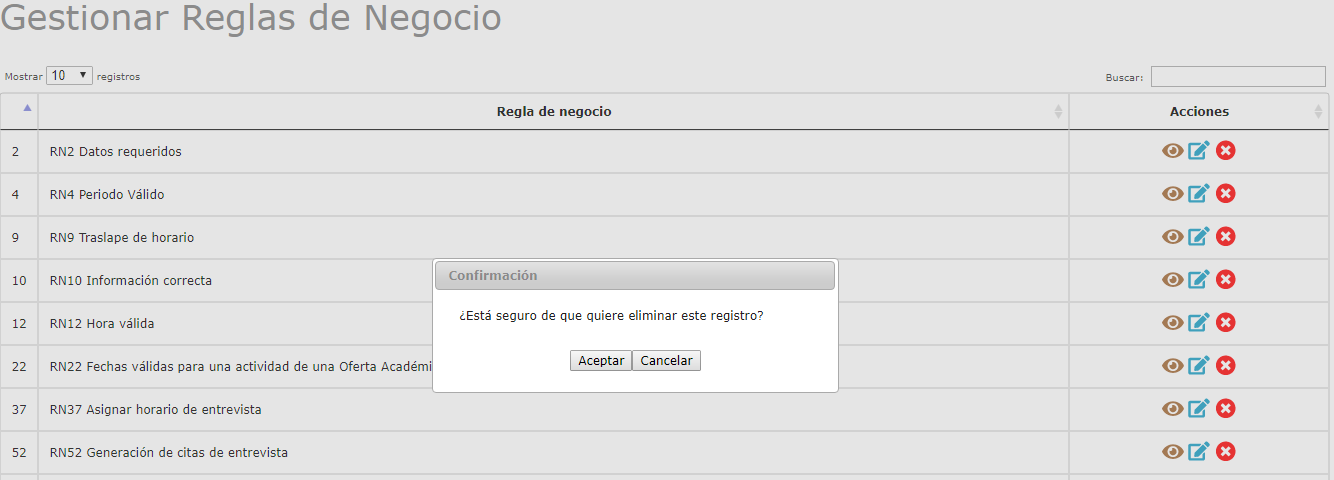
\includegraphics[scale=0.5]{roles/lider/reglasNegocio/pantallas/IU8-3MSG10}
					\caption{MSG de Confirmación}
					\label{fig:confirmaEliminaBR}
				\end{center}
			\end{figure}
						
			\item Oprima el botón \IUAceptar.
			
			\item Se mostrará el mensaje \ref{fig:BREliminada} en la pantalla \ref{fig:GestionarBR} ''Gestionar Reglas de negocio''.
			
			\begin{figure}[htbp!]
				\begin{center}
					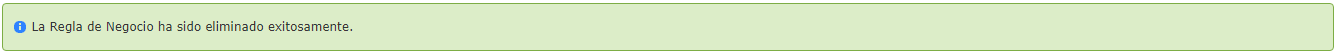
\includegraphics[scale=0.5]{roles/lider/reglasNegocio/pantallas/IU8-3MSG1}
					\caption{MSG: Regla de Negocio Eliminada}
					\label{fig:BREliminada}
				\end{center}
			\end{figure}
			\end{enumerate}